\newpage
\section{\Large EINLEITUNG}
Die in diesem Dokument beschriebene Software ist eine Modellier-Software, die dazu imstande ist, Körper und Flächen zu erstellen. Außerdem lassen sich die erstellten Modelle als OBJ-Datei speichern. Gespeicherte Modelle können geladen und auch bearbeitet werden.\newline
Zur Erstellung der Software wurde die Programmiersprache C/C++ genutzt unter Verwendung von OpenGL und ist sowohl mit Linux als auch Windows kompatibel.

\section{\Large BEDIENUNG}
\begin{labeling}[]{\textbf{Gewichtung der ausgewählte Punkte:}}%längster Wert
\item [\textbf{OBJ-Datei laden:}] \textbf{File} $\rightarrow$ \textbf{Open} oder \textbf{Strg + O}
\item [\textbf{Neues Objekt:}] \textbf{File} $\rightarrow$ \textbf{New} oder \textbf{Strg + N}
\item [\textbf{Objekt als OBJ speichern:}] \textbf{File} $\rightarrow$ \textbf{Save} oder \textbf{Strg + S}
\newline
\item [\textbf{Kamera Position verändern:}] '\textbf{w}', '\textbf{a}', '\textbf{s}', '\textbf{d}', '\textbf{q}', '\textbf{e}' - Tasten
\item [\textbf{Kameraausrichtung ändern:}] \textbf{linke Maustaste} + bewegen der Maus
\newline
\item [\textbf{Raster de/aktivieren:}] '\textbf{g}' - Taste
\item [\textbf{Punkte de/aktivieren:}] '\textbf{p}' - Taste
\item [\textbf{Kanten de/aktivieren:}] '\textbf{k}' - Taste
\newline
\item [\textbf{Punkt/e auswählen:}] \textbf{Strg} + Klick auf Punkt
\item [\textbf{Neuer Punkt:}] \textbf{rechte Maustaste} auf Raster oder Objekt
\item [\textbf{Ausgewählte Punkte löschen:}] '\textbf{r}' - Taste
\item [\textbf{Ausgewählte Punkte verschieben:}] Pfeiltasten, '\textbf{+}' und '\textbf{-}'
\newline
\item [\textbf{Erstellung eines Face:}] Punkte gegen Uhrzeigersinn auswählen + '\textbf{f}' - Taste
\newline
\item [\textbf{Catmull-Clark Unterteilung:}] '\textbf{c}' - Taste je Schritt
\item [\textbf{Unterteilung zurücksetzen:}] '\textbf{Strg + Z}
\newline
\item [\textbf{Gewichtung der ausgewählte Punkte:}] \textbf{Vertex} $\rightarrow$ \textbf{VertexWeight}
\newline
\item [\textbf{Smoothing:}] '\textbf{l}' - Taste je Schritt
\end{labeling}

\section{\Large SHADER}
Das Programm verwendet einen \textbf{Vertex Shader} und einen \textbf{Fragment Shader} für die Umsetzung des \textbf{Phong-shadings}. In die Beleuchtungs-Berechnung fließen die Position der primären Lichtquelle, die Farbe dieser Lichtquelle sowie weitere Faktoren wie die Farbe und Stärke des Umgebungslichtes und die Eigenschaften des Materials hinsichtlich der Spiegelungen. In Abhängigkeit des Betrachtungswinkels wird die Beleuchtung berechnet, indem die Normalen an den Vertices interpoliert werden. Außerdem werden mithilfe der Shader die Vertices als Kreise dargestellt.\newline\newline
Vorhergegangene Versuche zeigten deutlich, dass die Darstellung der Vertex-Punkte nicht effizient gelöst werden kann, wenn jeder Punkt durch ein eigenes VAO repräsentiert wird. Im Zuge dieser Erkenntnis entschloss sich das Team die Punkte darzustellen, indem alle Vertices mithilfe des Parameters GL\_POINTS als Point-Cloud gerendert werden. Diese Lösung ist effizient, jedoch ergab sich das Problem, dass die Punkte mit GL\_POINTS als Vierecke gerendert wurden. Die Lösung für dieses Problem besteht darin einen Radius zu definieren und alle Fragmente, die sich Außerhalb dieses Radius befinden, nicht zu rendern. Da die Größe dieser Kreise nicht in Raumkoordinatengrößen definiert werden, sondern in Pixelgröße, wurden die Punkte alle gleich groß, unabhängig von der Entfernung, gerendert. Um eine dynamische Größe zu gewährleisten, wird die Entfernung der Kamera zu dem Punkt berechnet und der Radius des Punktes wird proportional zur Entfernung kleiner.

\section{\Large KAMERA}
Um das Betrachten des Objektes von allen Seiten zu ermöglichen, entschied sich das Team eine Lösung zu implementieren, die \textbf{Quaternionen} nutzt. So wurde eine computerspielartige Steuerung der Kamera entwickelt, welche es ermöglicht die Ausrichtung der Kamera mithilfe der Maus zu beeinflussen und die Position der Kamera mithilfe der Tasten w, a, s, d, q und e zu verändern. Beim Drücken der linken Maustaste und Ziehen in eine Richtung wird eine Achse definiert, welche senkrecht zu der gezogenen Bahn steht. Um diese Achse wird die Ausrichtung der Kamera während der Bewegung rotiert.

\section{\Large CATMULL-CLARK UNTERTEILUNG}
Beim Catmull-Clark-Algorithmus werden beliebige Polygon-Gitter in Quad-Gitter unterteilt. Jedes n-Gon wird in n-Quads unterteilt. Zunächst wird für jedes Face ein Face-Punkt gesetzt, dieser wird aus dem Durchschnitt der Ausgangspunkte des jeweiligen Faces berechnet. Danach wird für jede Kante ein Kanten-Punkt hinzugefügt, der anhand der jeweiligen Endpunkte und der Nachbar Face Punkte und ebenfalls aus dem Durchschnitt dieser Punkte berechnet wird. Jeder neu berechnete Vertex wird mit den neu berechneten Kanten verbunden und weiter mit den Ausgangsvertices verbunden. Wenn das Ausgangsquad bereits zu einem Quad-Gitter unterteilt wurde, wird es erneut in vier weitere Quads unterteilt. Je öfter man den Algorithmus anwendet, desto feiner wird das Mesh.

\subsection{Limitpunkte und Limitnormalen}
Bei unendlich ofter Anwendung der Unterteilungsregeln auf ein Mesh wird die Limitfläche erzeugt. Durch Anwendung der Limitpunktregeln lässt sich für jeden Kontrollpunkt eines Kontrollgitters der entsprechende Punkt auf der Limitfläche bestimmen. Die Normale eines Limitpunktes erhält man durch das Kreuzprodukt der Oberflächentangenten an ebendieser Stelle des Limitpunktes.\\
In der Implementierung wird mit der Berechnung der Limitpunkte begonnen, nachdem man die Kontrollpunkte des neuen Meshes durch einen Unterteilungsschritt erhalten hat. Nun wird für jeden einzelnen Kontrollpunkt die Limitpunktregel angewandt. Dazu wird zunächst überprüft, ob und wie viele scharfe Kanten/Ränder mit dem Kontrollpunkt verbunden sind und entsprechend die Regel für glatte oder scharfe Kanten verwendet. Die Informationen über Valenz k und 1-Nachbarschaft erhält man durch geschicktes Manövrieren innerhalb der Halfedge-Datenstruktur.
%für glatte Kanten

\section{\Large ARCHITEKTUR}

\begin{figure}[H]
\centering
\includegraphics[width=0.7\linewidth]{uebersicht.png}
\caption{Übersicht}
\label{fig1}
\end{figure}

\subsection{GLWidget}

\begin{figure}[H]
\centering
\includegraphics[width=0.7\linewidth]{GLWidget.png}
\caption{GLWidget}
\label{fig2}
\end{figure}

Die Klasse \textbf{GLWidget} erweitert die QT-Klasee \textbf{QGLWidget} und gibt Funktionen wie das Laden einer OBJ-Datei oder das Speichern einer OBJ-Datei, sowie das Setzen der Vertex-Gewichtung an den MeshWrapper weiter.\newline\newline

\begin{labeling}[]{[\textbf{getWorldCoodinates()}}%längster Wert
\item[\textbf{initializeGL()}] OpenGL Funktionalitäten werden initialisiert, Kamera wird konfiguriert und Renderer wird mit seinem Shader-Programm geladen.
\item[\textbf{paintGL()}] Diese Funktion wird von QT in einer Rendering-Schleife aufgerufen, aktualisiert die Attribute der Kamera und bindet die aktuellen Matrizen, die von dem Shader benötigt werden, an den Shader.
\item[\textbf{mousePressEvent()}] Durch das Drücken einer Maustaste ausgelöst, führt die Aktionen \textbf{Vertex-Auswahl} und \textbf{Vertex-Erzeugung} aus. Beide Aktionen bedienen sich der Funktion \textbf{getWorldCoordinates()}.
\item[\textbf{getWorldCoodinates()}] implementiert Ray-Picking verfahren mithilfe der Funktionen \textbf{gluUnProject()} und \textbf{glReadPixels()}. In dem Ray-Picking Verfahren wird ein Strahl durch die 3D-Welt zwischen Near- und Far-Pane projiziert. Die Koordinaten im 3D-Raum an denen zuerst ein gerendertes Objekt gekreuzt wird, werden als Rückgabewert der Funktion \textbf{getWorldCoordinates()} zurückgeliefert. Aus diesem Grund bestand die Notwendigkeit eine Fläche in der 3D-Welt zu rendern, die von einem Raster überlagert wird. Diese Fläche ermöglicht es Vertices per Mausklick mittels des Ray-Picking-Verfahren hinzuzufügen. Die Fläche und das Raster können ausgeblendet werden, wenn sie beispielsweise bei der Betrachtung oder der Bearbeitung eines Objektes stören.
\item[\textbf{keyPressEvent()}] behandelt weitere Benutzerinteraktionen wie die Bewegung durch den Raum oder die Manipulation des Mesh und gibt diese an die jeweiligen Klassen weiter.
\end{labeling}

\subsection{Camera}

\begin{figure}[H]
\centering
\includegraphics[width=0.7\linewidth]{camera.png}
\caption{Camera}
\label{fig3}
\end{figure}

\begin{labeling}[]{[\textbf{changeHeading()}}%längster Wert
\item[\textbf{move()}] verändert die Position der Kamera und definiert die Richtung in die, die Kamera sich bewegt bei den jeweiligen Tasteneingaben.
\item[\textbf{changePitch()}] sorgt für die Drehung der Kamera und überprüft den Grad, um die sich die Kamera wenden soll mit einem Maximalwert um so die Geschwindigkeit einzuschränken.
\item[\textbf{changeHeading()}] bestimmt die Richtung der Fortbewegung.
\item[\textbf{move2D()}] berechnet anhand der vorherigen Mausposition die Drehung und Fortbewegungsrichtung der Kamera durch die Maus.
\item[\textbf{update()}] Diese Funktion aktualisiert und adaptiert die Kamera und dessen Attribute wie z. B. die Richtung, Drehung und Bewegung der Kamera.
\end{labeling}

\subsection{Catmull-Clark}

\begin{figure}[H]
\centering
\includegraphics[width=0.7\linewidth]{CatmullClark.png}
\caption{Catmull-Clark}
\label{fig4}
\end{figure}

\begin{labeling}[]{[\textbf{calc\_face\_centroid\_weighted()}}%längster Wert
\item[\textbf{operator()}] Zunächst werden die Gewichte auf 0 gesetzt, wodurch die Kanten geglättet werden. Danach werden n-Unterteilungen durchgeführt und für jedes Face wird die Mitte berechnet. Dann werden die Positionen der neuen Kantenpunkte berechnet. Darauf folgt die mittige Teilung jeder Kante.
\item[\textbf{calc\_face\_centroid\_weighted()}] berechnet das Zentrum eines Faces anhand seiner Vertices.
\item[\textbf{compute\_midpoint()}] berechnet den Mittelpunkt einer Kante anhand der Endpunkte dieser Kante und den Nachbarkanten.
\item[\textbf{update\_vertex()}] berechnet die neuen Positionen für die alten Vertices.
\item[\textbf{split\_face()}] Teilt ein n-Gon in n-Quads durch die Verbindung der neu erzeugten Vertices.
\item[\textbf{split\_edge()}] erstellt für die Mitte einer Kante einen neuen Vertex, dieser wird mit den Endpunkten neu verbunden.
\end{labeling}

\subsection{Object}

\begin{figure}[H]
\centering
\includegraphics[width=0.7\linewidth]{object.png}
\caption{Object}
\label{fig5}
\end{figure}

\noindent Die Klasse \textbf{Object} wird im Renderer benötigt. Hier werden alle Daten zu einem Objekt, welches gerendert werden soll, gespeichert. Die Daten bestehen aus den ID´s der unterschiedlichen Buffer-Objects, der ID des Vertex-Array-Objektes, sowie den Daten die dieses Objekt definieren. Der Renderer ist so Implementiert das nicht zwangsläufig alle Attribute des Objekts definiert sein müssen. Beispielsweise wird davon ausgegangen, dass die Vertices in Triangulierter-Form und Reihenfolge im vertex\_position\_buffer vorliegen, wenn der vertex\_index\_buffer nicht definiert ist.

\subsection{Renderer}

\begin{figure}[H]
\centering
\includegraphics[width=0.7\linewidth]{renderer.png}
\caption{Renderer}
\label{fig6}
\end{figure}

\noindent In dieser Klasse werden alle Operationen ausgeführt, die den Rendering-Prozess betreffen. Die Klasse hält verschieden Instanzen der Object Struktur. Das Mesh wird in dreifacher Variation als Object gehalten:
\begin{enumerate}
\item für die Darstellung der Flächen
\item für die Darstellung der Punkte
\item für die Darstellung der Linien, die die Kanten der Faces visualisieren.
\end{enumerate}
Außerdem werden Objects für das Raster sowie die Fläche unterhalb des Rasters initialisiert.\newline
Bei der Initialisierung der einzelnen Objekte werden die Daten-Attribute der Object Instanz belegt und für jedes Objekt wird ein VAO erstellt sowie die buffer\_objects der Daten-Attribute, die belegt sind, werden erzeugt. Hierfür werden die Template-Funktion \textbf{setup\_buffer\_data()} und \textbf{bindBufferToShader()} verwendet. \textbf{updateBufferData()} ist eine Template-Funktion, welche \textbf{glBufferSubData} nutzt, um die gespeicherten Daten zu aktualisieren. Dies geschieht zum Beispiel, wenn ein Vertex-Punkt verschoben wird. Wird ein Punkt hinzugefügt, entfernt oder ein Face erstellt, wird die Größe des Buffer-Objects verändert. Für diesen Fall eignet sich \textbf{glBufferSubData} nicht mehr und die entsprechende Buffer-Objects werden mittels \textbf{recreateMesh()} neu erstellt.\newline
Bei der Initialisierung der Renderer Instanz werden die Dimensionen des Mesh-Objektes berücksichtigt. Es werden die minimalen und maximalen Vertex-Positionen ermittelt und das Raster-Objekt wird unterhalb der niedrigsten Position auf der Y-Achse positioniert. Zusätzlich wird das Raster auf eine Größe, die 50\% größer als die Differenz aus der Maximalen X und Minimalen X Position oder, wenn diese größer ist, die Differenz auf der Z-Achse, beschränkt.

\subsection{Shader}

\begin{figure}[H]
\centering
\includegraphics[width=0.7\linewidth]{shader.png}
\caption{Shader}
\label{fig7}
\end{figure}

\noindent Die Shader-Klasse bindet die übergebenen zwei GLSL-Shader an die Grafikkarte. Hierfür werden die übergebenen Shader ausgelesen und die benötigten Parameter an die Shader weitergeleitet. In unserem Programm beschränken wir uns auf die Verwendung eines \textbf{Vertex-Shaders} und eines \textbf{Fragment-Shaders}, welche das \textbf{Phong-Shading} umsetzen und für die korrekte Darstellung der Punkte zuständig sind.

\subsection{MeshWrapper}

\begin{figure}[H]
\centering
\includegraphics[width=0.7\linewidth]{meshWrapper.png}
\caption{Meshwrapper}
\label{fig8}
\end{figure}

\noindent Der \textbf{MeshWrapper} schachtelt die OpenMesh-Funktionalitäten und schafft eine Schnittstelle um die Interaktion mit dem Mesh zu ermöglichen. Für die Konfiguration des Meshes wird ein struct verwendet, welches festlegt, dass die Punkte und Normalen als float gespeichert werden. Somit ist die Integration in die Umgebung, welche vorwiegend mit dem Datentyp float arbeitet gewährleistet. Da für die Gewichtung der Vertices bei der Berechnung der Unterteilungsflächen eine vierte Komponente benötigt wird, wird die Klasse \textbf{HE\_MESH} genutzt, welche von der Klasse PolyMesh, aus der OpenMesh-Bibliothek, abgeleitet wird.\newline
Der MeshWrapper verfügt über ein Objekt der Klasse \textbf{HE\_MESH}. Dieses Objekt repräsentiert das Mesh. Außerdem wird ein std::vector verwendet der die aktuell markierten Vertices speichert. Zudem wird ein Backstack angelegt, der bei jeder Ausführung des Catmull-Clark Unterteilungsflächen-Algorithmus, das Mesh speichert. Dadurch kann jeder Unterteilungsschritt rückgängig gemacht werden.\newline
Für die Verwendung im Renderer liefert die Funktion \textbf{getVerticesAndNormalsTriangulated()} eine Triangulierte Version des Meshes. Hierfür werden alle Faces durchlaufen und jeder dem aktuellen Face zugehöriger Vertex wird in einem std::vector gespeichert.\newline
Für die Darstellung der Kanten werden alle Kanten des Meshes durchlaufen und die Anfangs-, sowie End-Vertices in einem std::vector gespeichert.\newline
Um einen Vertex auszuwählen, werden die Welt-Koordinaten die, in der Klasse GLWidget bestimmt wurden an die Funktion \textbf{selectVertex()} übergeben. Hier werden nun alle Vertices überprüft, ob diese auf den Koordinaten liegen. In diesem Prozess wird eine kleine Abweichung toleriert. Ist der angeklickte Vertex schon in der Liste, wird er entfernt.

\newpage

	\section{\Large ALGORITHMEN}

\subsection{Kamera}

\begin{lstlisting}

projection = glm::perspective(glm::radians(field_of_view), aspect, near_clip, far_clip);

/*
* Achse für Pitch-Rotation festlegen
*/
glm::vec3 axis = glm::cross(camera_direction,glm::vec3(0.0f, 1.0f, 0.0f););

/*
* Quaternion für Pitch auf Basis des Kamera-Pitchwinkels berechnen
* Pitch wird durch Mausbewegung in horizontaler Richtung beeinflusst
*/
glm::quat pitch_quat = glm::angleAxis(camera_pitch, axis);

/*
* Bestimmung des Heading-Quaternions aus dem Kamera-Aufwärtsvektor und dem Heading-Winkel
* heading wird durch Mausbewegung in vertikaler Richtung beeinflusst
*/
glm::quat heading_quat = glm::angleAxis(camera_heading, glm::vec3(0.0f, 1.0f, 0.0f););

/*
* Kreuzprodukt der beiden Quaternionen, normalisieren
*/
glm::quat temp = glm::cross(pitch_quat, heading_quat);
temp = glm::normalize(temp);

/*
* die Richtung der Kamera mit der Quaternion aktualisieren
*/
camera_direction = glm::rotate(temp, camera_direction);

/*
* Kamera position aktualisieren
*/
camera_position += camera_position_delta;

/*
* lookAt aktualisieren
*/
camera_look_at = camera_position + camera_direction * 1.0f;

\end{lstlisting}

\subsection{Smoothing}

Die Glättung wird erreicht, indem jeder Vertex an die Position verschoben wird, die dem Durchschnittswert seiner benachbarten Vertices entspricht. Um dies zu erreichen werden die neuen Positionen der Vertices zwischengespeichert. Nachdem jeder Vertex neu errechnet wurde, werden die alten Werte durch die zwischengespeicherten Werte ersetzt.

\[\overline{x}_i = \frac{1}{N}\sum_{j=1}^{N}\overline{x}_j\]
wobei \(\overline{x}_i\) die neue Position des Vertex und N die Anzahl der benachbarten Vertices ist.

\subsection{Shader}

\subsubsection{Vertex Shader}

\begin{lstlisting}
vec4 vertex = vec4(vertex_position, 1.0);

/*
* Transformation der Normale und der Position für den Fragmentshader
*/
normal = normalize(normalMatrix * vertex_normal);
position = vec3(viewMatrix * modelMatrix * vertex);

/*
* Grundfarben ändern sich nicht pro Pixel - können jetzt berechnet werden
*/
ambient = materialAmbient * lightAmbient;
diffuse = materialDiffuse * lightDiffuse;
ambientGlobal = materialAmbient * lightGlobal;

/*
* Dynamische Anpassung der Punktgröße abhängig von der Entfernung der Kamera
*/
float distance = length(vertex_position - cameraPos);
gl_PointSize = radius_attr/distance;

/*
* Vertex-Position in OpenGL setzen
*/
gl_Position = projectionMatrix * viewMatrix * modelMatrix * vertex;

\end{lstlisting}

\subsubsection{Fragment Shader}

\begin{lstlisting}
/*
* Lichtberechnung
*/
vec3 N = normalize(normal);
vec3 L = normalize(lightPosition - position);
vec3 R = 2 * dot(L, N) * N - L;

float cosTheta = max(dot(L, N), 0.0);
float cosAlpha = max(dot(N, R), 0.0);

float attenuation = 1.0 / (constantAttenuation + length(L) * linearAttenuation);

vec3 tempColor = VertexIn.vertex_color + ambientGlobal;

if (cosTheta &gt; 0.0) {
tempColor += attenuation * (diffuse * cosTheta + ambient);
tempColor += attenuation
* materialSpecular
* lightSpecular
* pow(cosAlpha, materialShininess);
}

/*
* ist das Radius-Attribut gesetzt, handelt es sich um einen Punkt
*/
if(VertexIn.radius &gt; 0){
vec3 N;
N.xy = gl_PointCoord * 2.0 - vec2(1.0);
float mag = dot(N.xy, N.xy);

/*
* Pixel außerhalb des Kreises werden nicht dargestellt
*/
if (mag &gt; 1.0) discard;

N.z = sqrt( 1.0 - mag);
}

/*
* Pixelfarbe in OpenGL setzen
*/
color = vec4(tempColor, 1.0);

\end{lstlisting}

\subsection{Catmull und vierte Komponente}

Durch Nutzung der OpenMesh Bibliotheken wurden neben den vielen Vorteilen welche sie liefern einige Einschränkungen auferlegt. So können die Implementierungen des ArrayKernels nur mit Typen von Punkten arbeiten, welche drei Komponenten haben. Um diesen nicht vollständig neu implementieren zu müssen, entschieden wir uns eine sogenannte ``property'' zu nutzen. Diese beschreibt eine weitere Variable die jeder Vertex zusätzlich zwischenspeichert. So können wir die Gewichte für die ausgewählten Punkte setzen um diese später im Catmull-Clark Algorithmus mit in die Rechnung aufnehmen zu können.

\begin{lstlisting}
struct Traits : OpenMesh::DefaultTraits
{
    // Let Point and Normal be a float vec3
    typedef OpenMesh::Vec3f Point;
    typedef OpenMesh::Vec3f Normal;

};


class HE_MESH : public OpenMesh::PolyMesh_ArrayKernelT<Traits> {
public:
    HE_MESH() {
        this->add_property(this->vp_fourth);
    }
    OpenMesh::VPropHandleT<float> vp_fourth;
};
\end{lstlisting}

\section{\Large PROBLEME UND LÖSUNGEN}
Um zu Beginn möglichst schnell einen Prototyp zu entwickeln, der das Testen und weiterarbeiten vereinfacht, setzte unser Team anfänglich auf die Verwendung des alten OpenGL Kontextes, der es ermöglicht direkt zu rendern ohne die Verwendung von Shadern und VAO, VBO, etc. Dieser Prototyp verwendete eine überarbeitete Version der Half-Edge Datenstruktur aus dem 4. Semester. Mit dem Prototyp konnten alle Anforderungen der ersten Milestones erfüllt werden. \newline
Da die eigene Half-Edge Datenstruktur nicht über die Möglichkeit verfügte Vertices oder Faces zu löschen, entschieden wir uns für die Verwendung der OpenMesh Half-Edge-Datenstruktur.\newline
Um unseren Ansprüchen Genüge zu tun, endschieden wir uns auf einen aktuellen OpenGL Kontext umzusteigen. Dieser Umstieg erforderte es ein völlig neues Projekt zu erzeugen, da wir viele Dinge selber implementieren mussten, die vorher nicht notwendig waren. Beispielsweise die Darstellung der Punkte, welche sich im Prototyp auf die Nutzung der GLUT-Funktion glutSolidSphere() beschränkte, wurde zu einem umfangreicheren Unterfangen. Trotz einiger Schwierigkeiten und der Erzeugung von Mehraufwand bereuen wir diesen Schritt jedoch nicht, da wir unser Wissen aus dem ersten Computergrafik-Modul auffrischen konnten, was nötig und hilfreich für das Verständnis einiger Themen aus dem aktuellen Kurs war.\newline
Als Entwicklungsumgebung setzten wir auf die IDE „CLion“ und achteten darauf das wir unabhängig vom Betriebssystem sind, um mit Windows sowie Linux an dem Projekt arbeiten zu können. Hierbei wurden wir vor einige Herausforderungen, mit welchen wir so nicht gerechnet hatten, gestellt. Diese Probleme beruhten zum großen Teil auf der Kompatibilität der Toolchain der einzelnen Module. So mussten wir die meisten Bibliotheken, die wir verwenden, selber kompilieren und hatten dennoch Schwierigkeiten ein fehlerfreies Zusammenspiel der Komponenten zu gewährleisten. Für zukünftige Projekte werden wir wahrscheinlich auf Visual-Studio und die Visual-Studio Toolchain setzen, da die meisten Bibliotheken im Computergrafik Bereich hierfür konfiguriert sind und so einiges an Problemen und Arbeit eingespart wird.

\section{\Large BENUTZEROBERFLÄCHE}

\begin{figure}[H]
\centering
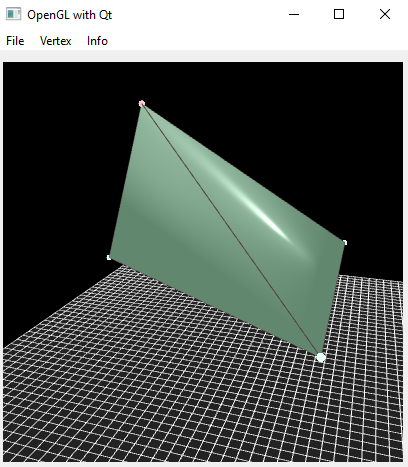
\includegraphics[width=0.7\linewidth]{GUI.png}
\caption{Benutzeroberfläche}
\label{fig9}
\end{figure}
	

	

		